\documentclass{ctexart}
%
%页眉页脚

\usepackage{geometry}
\geometry{left=2.5cm,right=2.5cm,top=2.5cm,bottom=2.5cm}

\usepackage{xcolor}
\usepackage{graphicx}
\usepackage{amsmath}
\usepackage{url}
\usepackage{enumerate}
\usepackage{subfigure}
\usepackage{listings} 
\usepackage[colorlinks,linkcolor=black]{hyperref}% 书签
\lstset{numbers=left, %设置行号位置
    numberstyle=\tiny, %设置行号大小
    keywordstyle=\color{blue}, %设置关键字颜色
    commentstyle=\color[cmyk]{1,0,1,0}, %设置注释颜色
    frame=single, %设置边框格式
    breaklines, %自动折行
    extendedchars=false, %解决代码跨页时,章节标题,页眉等汉字不显示的问题
    xleftmargin=1.5em,xrightmargin=1.5em, aboveskip=1em, %设置边距
    tabsize=4, %设置tab空格数
    showspaces=false %不显示空格
}
%中文
\usepackage{xeCJK}
%字体设置
\usepackage{indentfirst}
\setlength{\parindent}{2em} %首行缩进



\title{MATLAB 综合实验之音乐合成\footnote{所有的.m文件均采用utf8编码,在matlab中打开可能会出现中文乱码的情况,请用其它编辑器打开}}
\author{聂浩~~ 无31~~ 2013011280}
\date{\today}
\begin{document}
\maketitle
\section{简单的合成音乐}
\footnote{本部分在目录dfh中执行}
    \subsection{请根据《东方红》片断的简谱和“十二平均律”计算出该片断中各个乐音的频率,
            在 MATLAB 中生成幅度为 1 、抽样频率为 8kHz 的正弦信号表示这些乐音。请用 sound 函
            数播放每个乐音,听一听音调是否正确。最后用这一系列乐音信号拼出《东方红》片断,注
        意控制每个乐音持续的时间要符合节拍,用 sound 播放你合成的音乐,听起来感觉如何?}

        思路:利用12平均律的定义,并假设每拍为构造m\_ note函数,将音调和持续时间传过去\footnote{与输入的base相差的音阶,从-5到19共25个音,传-10表示这是空节拍},调用一次函数发一次音,这样只需要按照次序产生各个音即可。\footnote{这里参考了matlab help kron中的内容}

        听起来调子是对的,但是各个音之间有爆破音。

        代码如下(dfh\_1.m和m\_note\_1.,m):

        \lstinputlisting[language=matlab]{dfh/dfh_1.m}
        \lstinputlisting[language=matlab]{dfh/m_note_1.m}

    \subsection{
            你一定注意到 (1) 的乐曲中相邻乐音之间有“啪”的杂声,这是由于相位不连续产
            生了高频分量。这种噪声严重影响合成音乐的质量,丧失真实感。为了消除它,我们可以用
            图 1.5 所示包络修正每个乐音,以保证在乐音的邻接处信号幅度为零。此外建议用指数衰
            减的包络来表示。
        }

        思路:直接利用 .* 给生成的s信号乘以一个指数变换的序列来改变包络,使得每一个音看起来像图\ref{11},虽然开始结束时不严格为0,但是合理的参数设定使得这两个点的振幅非常接近0。
        为了方便处理,将每个音的产生和播放分开。将每个音节产生的音乐序列连在数组s后面,最后统一播放s。
        
        代码如下(dfh\_2.m和m\_note\_2.,m):

        \lstinputlisting[language=matlab]{dfh/dfh_2.m}
        \lstinputlisting[language=matlab]{dfh/m_note_2.m}


        \begin{figure}
            \centering
            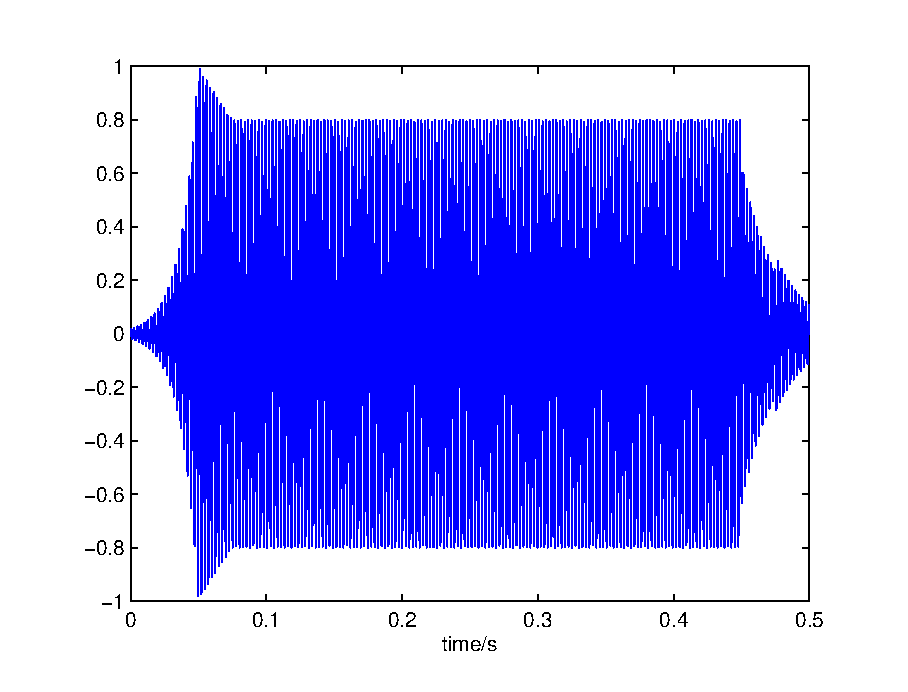
\includegraphics[width=0.8\textwidth]{dfh/1_1.eps}\\
            \caption{增加了包络的信号\label{11}}
        \end{figure}

        
        这里消除了爆音,但音色听起来有点奇怪。
    \subsection{
            请用最简单的方法将 (2) 中的音乐分别升高和降低一个八度。 (提示:音乐播放的
            时间可以变化)再难一些,请用 resample 函数(也可以用 interp 和 decimate 函数)将上述
            音乐升高半个音阶。 (提示:视计算复杂度,不必特别精确)
        }

        答:最简单的方法是改变播放时sound函数的采样率来进行播放,本质上是改变播放的速率。利用十二平均律的定义,利用上一问中得到的s,可以有:

        二倍速播放,高了一个八度
        \begin{lstlisting}[language=matlab]
        sound(s,16000)
        \end{lstlisting}
        即0.5倍速播放,低了一个八度。
        \begin{lstlisting}[language=matlab]
        sound(s,4000)
        \end{lstlisting}
        resample函数为修改函数的采样率,然后以原来的采样率播放,就会改变音调。提高半个音阶使s的采样率变为$\frac{8000}{2^{\frac{1}{12}}}$,然后仍然以8000的采样率播放即可,这样做依然会有播放时间改变的问题。具体做法为:

        \begin{lstlisting}[language=matlab]
        resample(s,10000,10594);
        sound(s,8000)
        \end{lstlisting}

        由于只改变了半个音阶,虽然没有对音乐的时间进行调整,但是听起来变化不大。

        思考:本题的思路比较简单,主要在于对resample函数使用和原理的了解。这里利用matlab 提供的文档以及搜索引擎进行学习也是掌握matlab函数的常规方法。

    \subsection{
            试着在 (2) 的音乐中增加一些谐波分量,听一听音乐是否更有“厚度”了?注意谐
            波分量的能量要小,否则掩盖住基音反而听不清音调了。 (如果选择基波幅度为 1 ,二次谐
            波幅度 0.2 ,三次谐波幅度 0.3 ,听起来像不像象风琴?)
        }

        思路:只需在产生每个音时把谐波加上就可以了,其他并不用改变,

				代码如下(dfh\_3.m,m\_note\_3.m)
        \lstinputlisting[language=matlab]{dfh/dfh_3.m}
        \lstinputlisting[language=matlab]{dfh/m_note_3.m}

        思考:听起来有点风琴的感觉,同时也挺像笛子,这和音的包络也有关系。

    \subsection{
        自选其它音乐合成,例如贝多芬第五交响乐的开头两小节。}

        思路:合成的是致爱丽丝的第二节。
        出于方便输入的考量,首先将标准的简谱和对应的音的时间长存在两个数组中,
        然后用matlab转换谱子为十二平均律的形式,再循环调用之前的m\_note\_3 函数代码如下(my\_music.m):
        \lstinputlisting[language=matlab]{dfh/my_music.m}

        波形图如图\ref{15}:
        \begin{figure}
            \centering
            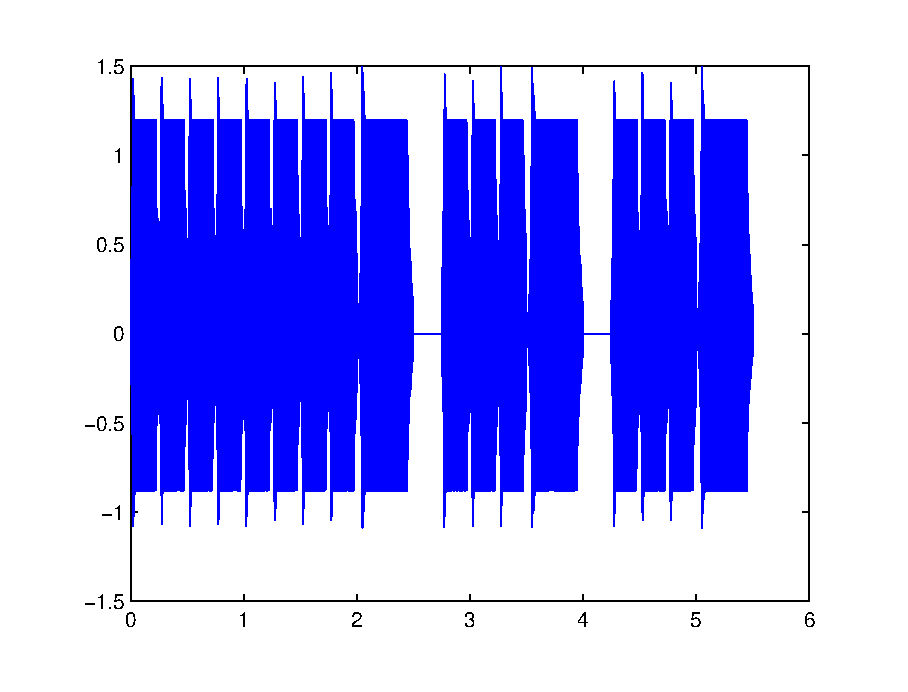
\includegraphics[width=0.8\textwidth]{dfh/1_5.eps}\\
            \caption{合成音乐波形图\label{15}}
        \end{figure}
        \section{用傅里叶级数分析音乐}\footnote{本部分在目录fmt中执行}
		\setcounter{subsection}{5} 
    \subsection{先用 wavread 函数载入光盘中的 fmt.wav 文件,播放出来听听效果如何?是否比刚
        才的合成音乐真实多了?}

        听起来是很明显的吉他声,确实真实很多。操作如下:
        \begin{lstlisting}[language=matlab]
        [R Fs]=audioread(fmt.wav);
        sound(R,Fs);
        \end{lstlisting}
    \subsection{
            你知道待处理的 wave2proc 是如何从真实值 realwave 中得到的么? 这个预处理过
            程可以去除真实乐曲中的非线性谐波和噪声, 对于正确分析音调是非常重要的。 提示: 从
        时域做, 可以继续使用 resample 函数。}

        思路:先对wave2proc和realwave做傅立叶分析,画出其频谱图如图\ref{161}.可以看出,两者的频谱除了低频部分基本是一致的,思路首先是滤去realwave的低频部分然后进行傅里叶逆变换。
        但题目要求以时域的方法处理,同时由于realwave中的低频分量不是很好处理,所以没有采用这种方案。

        傅立叶分析代码\footnote{这里参照了matlab fft demo的代码}(anay\_wave.m)
        \lstinputlisting[language=matlab]{fmt/anay_wave.m}
        \begin{figure}
            \centering
            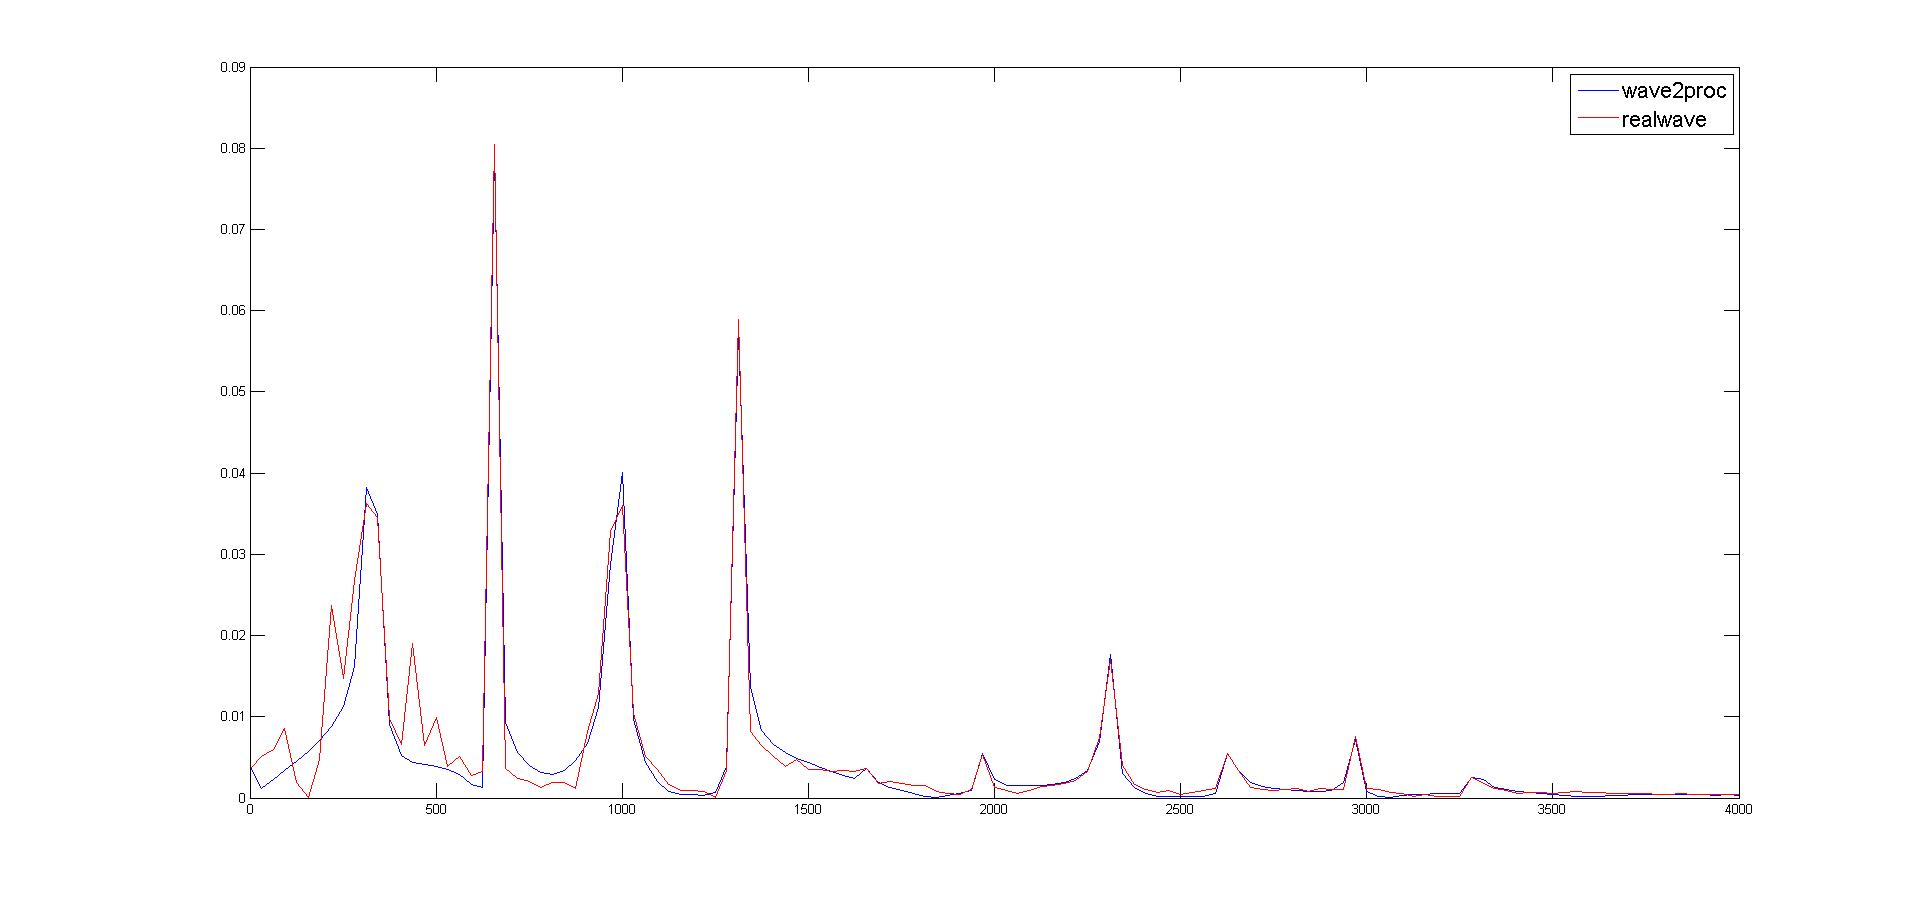
\includegraphics[width=0.8\textwidth]{fmt/1_6_1.jpg}
            \caption{wave2proc与realwave的频谱\label{161}}
        \end{figure}
        \begin{figure}
            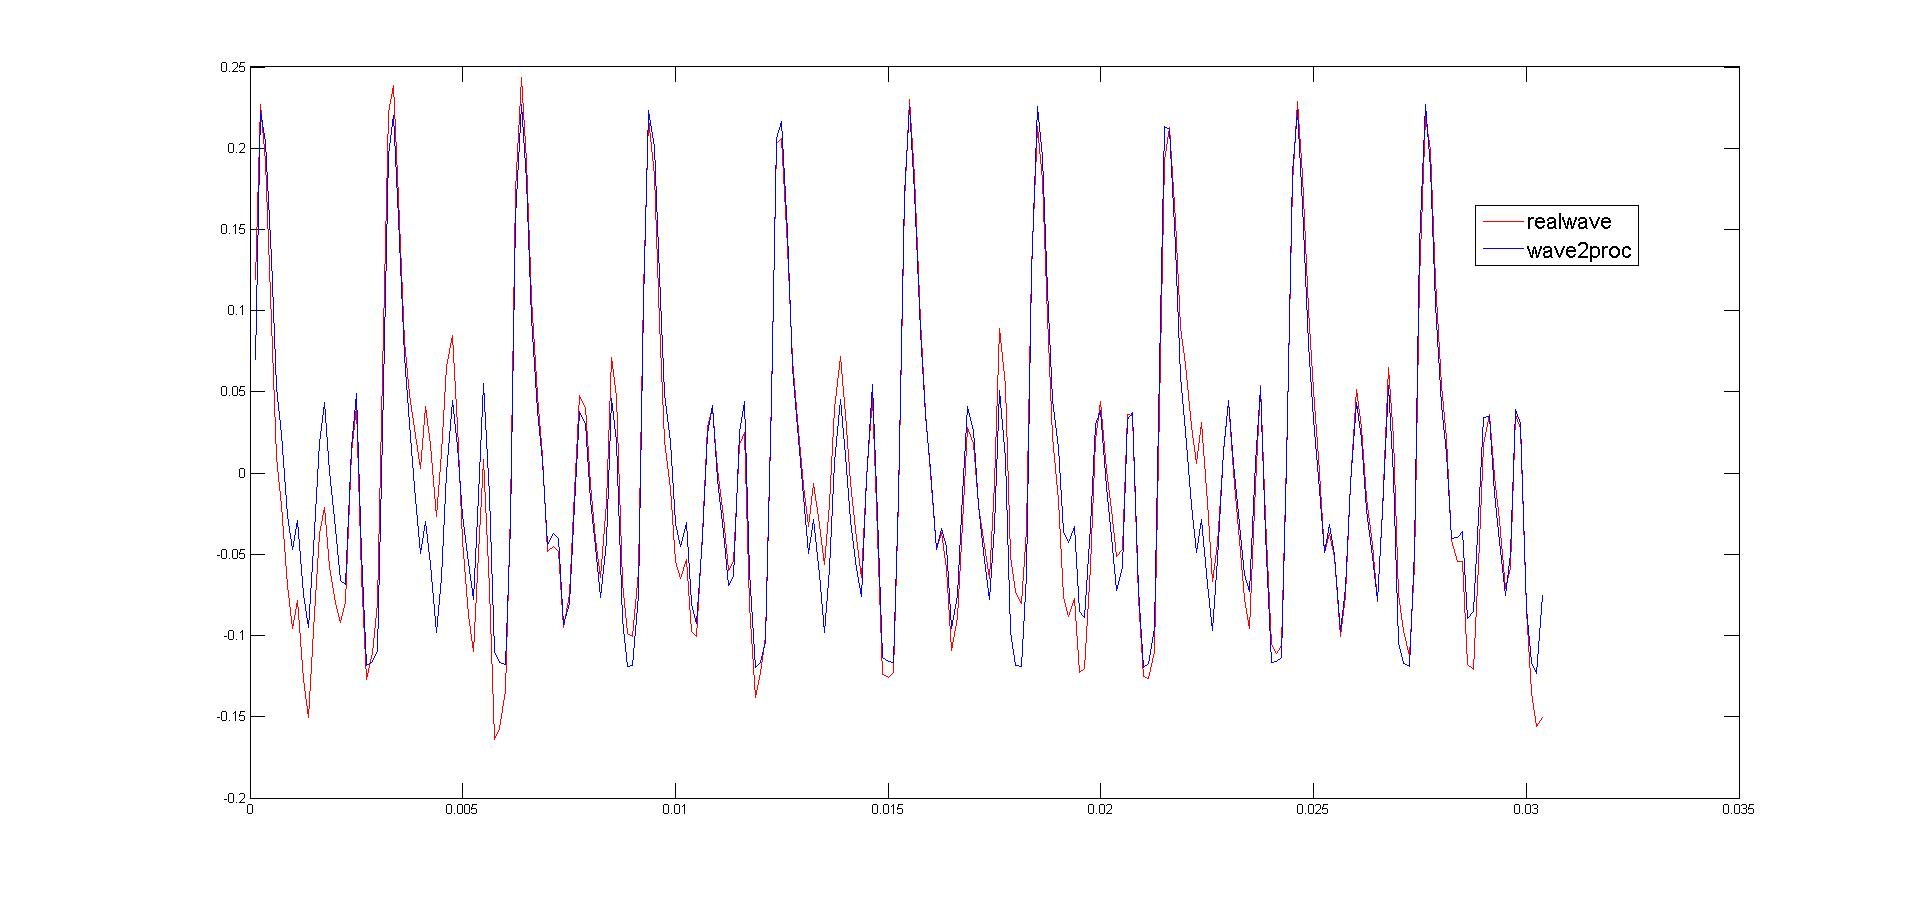
\includegraphics[width=0.8\textwidth]{fmt/1_6_2.jpg}
            \centering
            \caption{wave2proc与realwave的波形\label{162}}
        \end{figure}
        这里观察wave2proc和realwave的波形如图\ref{162}。可以看出,
        大致有十个峰。将wave2proc的十个峰画在一起如图\ref{163},其周期性相当强。
        因此将realwave分为10个周期,然后对其求平均得到一个周期,再延拓。
        需要注意的是,realwave有243个采样点,应先用resample函数将此采样为250个点,
        处理完后再恢复为243个。生成的波形如图\ref{164}

        \begin{figure}
            \centering
            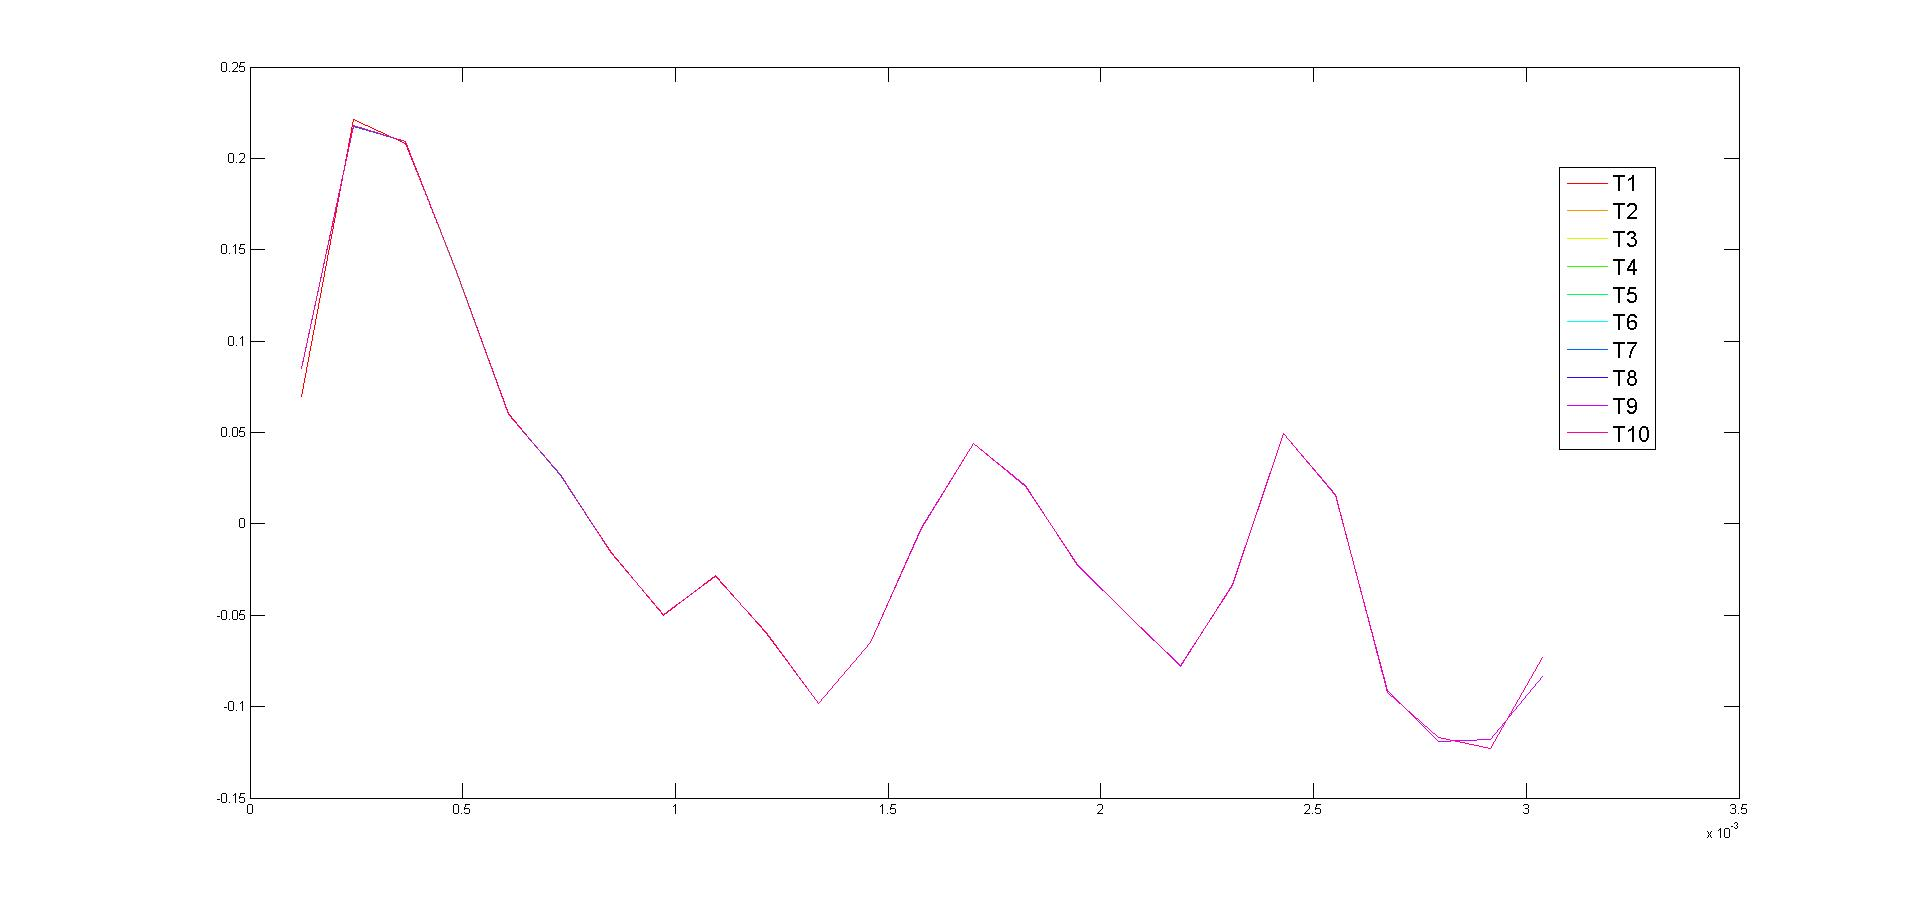
\includegraphics[width=0.8\textwidth]{fmt/1_6_3.jpg}\\
            \caption{wave2proc的十个周期\label{163}}
        \end{figure}
        \begin{figure}
            \centering
            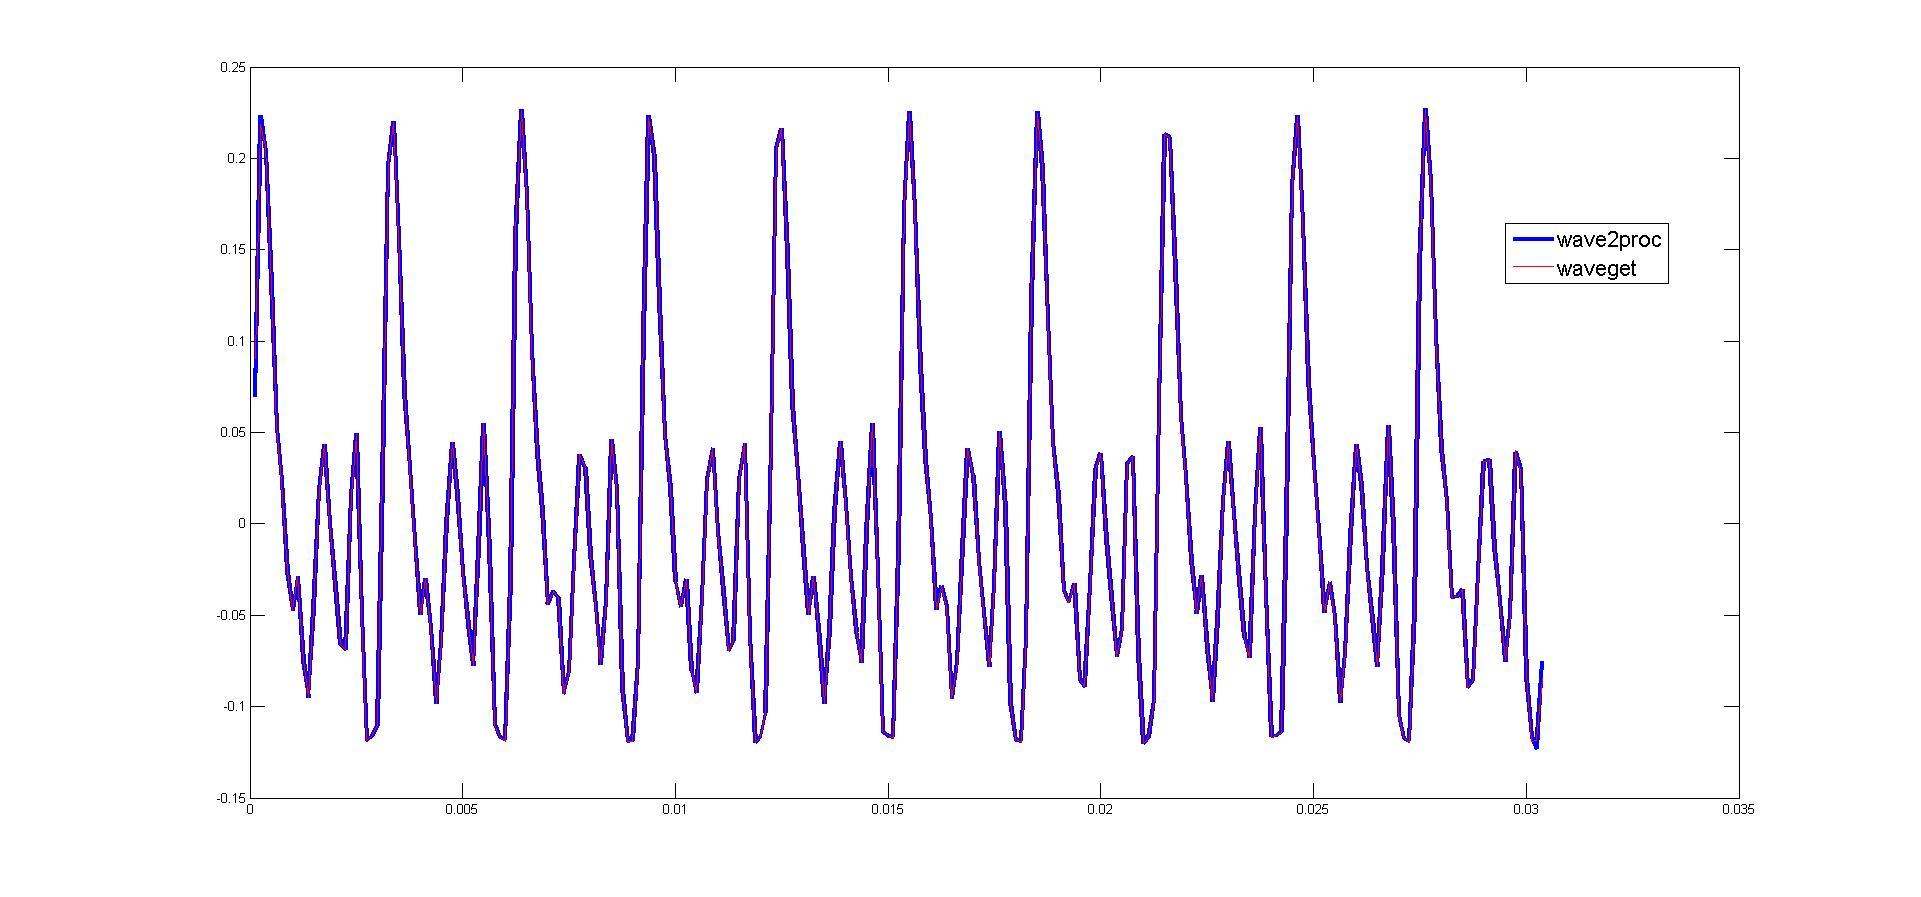
\includegraphics[width=0.8\textwidth]{fmt/1_6_4.jpg}\\
            \caption{wave2proc与得到的波形\label{164}}

        \end{figure}


        画图代码为
        \begin{lstlisting}[language=matlab]
        clc;clear;close all;
        Fs=8000;
        load guitar.mat;
        tmp=resample(wave2proc,250,243);
        t=(1:25)/(8000/243*250);
        colors= hsv(10);
        labels=[];
        for d=1:10
        plot(t,tmp((d-1)*25+1:d*25),'color',colors(d,:));
        labels{d}=['T' num2str(d)];
        hold on 
        end
        legend(labels);
        \end{lstlisting}

        波形生成代码(wave4proc.m)
        \lstinputlisting[language=matlab]{fmt/wave4proc.m}

        思考:所得到的波形和wave2proc是非常相似的,这样做通过平均减弱了噪音和多次谐波的影响。
    \subsection{
            这段音乐的基频是多少? 是哪个音调? 请用傅里叶级数或者变换的方法分析它的谐
            波分量分别是什么。 提示: 简单的方法是近似取出一个周期求傅里叶级数但这样明显不准
            确, 因为你应该已经发现基音周期不是整数( 这里不允许使用 resample 函数)。 复杂些的方
            法是对整个信号求傅里叶变换( 回忆周期性信号的傅里叶变换), 但你可能发现无论你如何
            提高频域的分辨率, 也得不到精确的包络( 应该近似于冲激函数而不是 sinc 函数), 可选的
            方法是增加时域的数据量, 即再把时域信号重复若干次, 看看这样是否效果好多了? 请解
            释之。
        }

        思路:将该段音乐重复100次后利用fft函数进行傅里叶变换如图\ref{18},得到表\ref{sheet1},分析得到基波为328.10Hz,
        对应E2(mi)的音。
				
        \begin{figure}
            \centering
            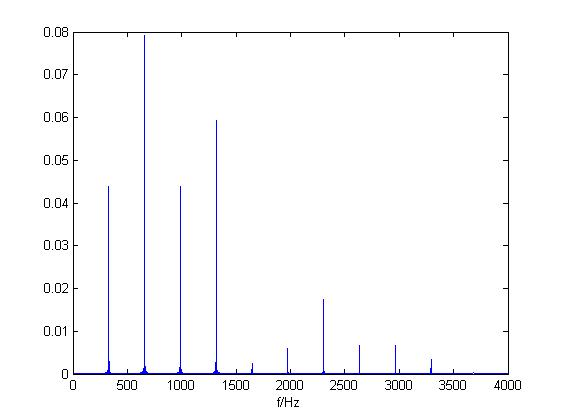
\includegraphics[width=0.8\textwidth]{fmt/1_8.jpg}\\
            \caption{wave2proc重复1000次后的频谱图\label{18}}

        \end{figure}
        
        \begin{table}
            \centering
            \begin{tabular}{|c|c|c|c|c|c|c|}
                \hline
                &基波&一次谐波&二次谐波&三次谐波&四次谐波&五次谐波\\
                \hline
                频率/Hz&329.10&658.40&987.26&1316.36&1645.22&1974.32\\
                \hline
                幅度&0.0439&0.0791&0.0438&0.0594&0.0025&0.0059\\
                \hline
                相对幅度\footnote{相对基波}&1&1.80&1.00&1.35&0.06&0.13\\
                \hline
            \end{tabular}
            \caption{realwave的基波及谐波\label{sheet1}}
        \end{table}

				代码如下(get\_base.m):
        \lstinputlisting[language=matlab]{fmt/get_base.m}

        思考:将图\ref{18}和图\ref{162}可以看出重复后的频谱图看起来更近似冲激串。
        这是因为时域上的延拓为是与信号与很多冲激函数分别卷积后再求和,
        当重复次数很多时,这一过程相当于在频域上对信号进行采样(采样间隔为$\frac{1}{T}=32.92Hz$),
        之一过程可以有效去除噪音和不规则谐波。
    \subsection{
            再次载入 fmt.wav ,现在要求你写一段程序,自动分析出这段乐曲的音调和节拍!
            如果你觉得太难就允许手工标定出每个音调的起止时间,再不行你就把每个音调的数据都
            单独保存成一个文件,然后让 MATLAB 对这些文件进行批处理。注意:不允许逐一地手工
            分析音调。编辑音乐文件,推荐使用“CoolEdit” 编辑软件。
        }

        思路:因为之前做过小白鲸找妈妈的作业,所以第一想法是对信号进行短时傅里叶变换\footnote{此处参照网络教程\url{http://blog.sina.com.cn/s/blog_6163bdeb0102dwfw.html}},然后每隔$\frac{1}{4}$拍读取一次频率,这样就可以得到各个时间点的音调,因为音乐约为16.3秒,约为32.5拍,所以分为140段进行短时傅里叶变换。变换结果如图\ref{191}.
        \begin{figure}
            \centering
            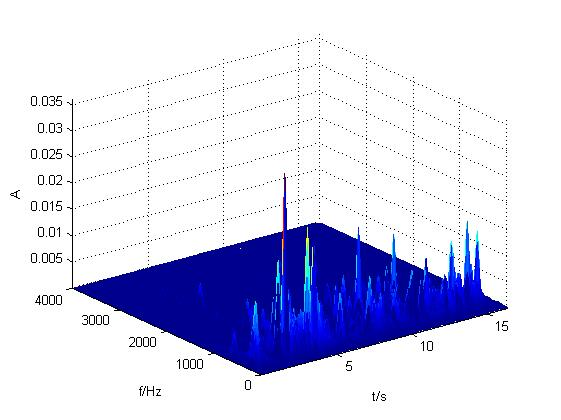
\includegraphics[width=0.8\textwidth]{fmt/1_9_1.jpg}\\
            \caption{fmt音乐的时频图\label{191}}
        \end{figure}


        代码是这样的(short\_fourier.m)
        \lstinputlisting[language=matlab]{fmt/short_fourier.m}

        然而很难分清得到的4分音符究竟是独立的一个音还是和前后的音连在一起的长音。需要分析音乐的节拍。方案有:
        \begin{itemize}
            \item{提取音乐的包络,但是在用高斯滤波提取后,
                得到的波形图与原波形契合度不高,无法获得音节划分。}
            \item{仿照cooledit节拍分化的功能,通过判断时域信号在短时间(指定时间,取6ms)
                    内的变化率(取6.5dB临界值)进行节奏分化。但是如图\ref{192}所示,
                    12.37s时幅度变化太小,小于一些拍子内部的变化,无法划分。在调整参数后,
                也无法解决该问题}
        \end{itemize}
        \begin{figure}
            \centering
            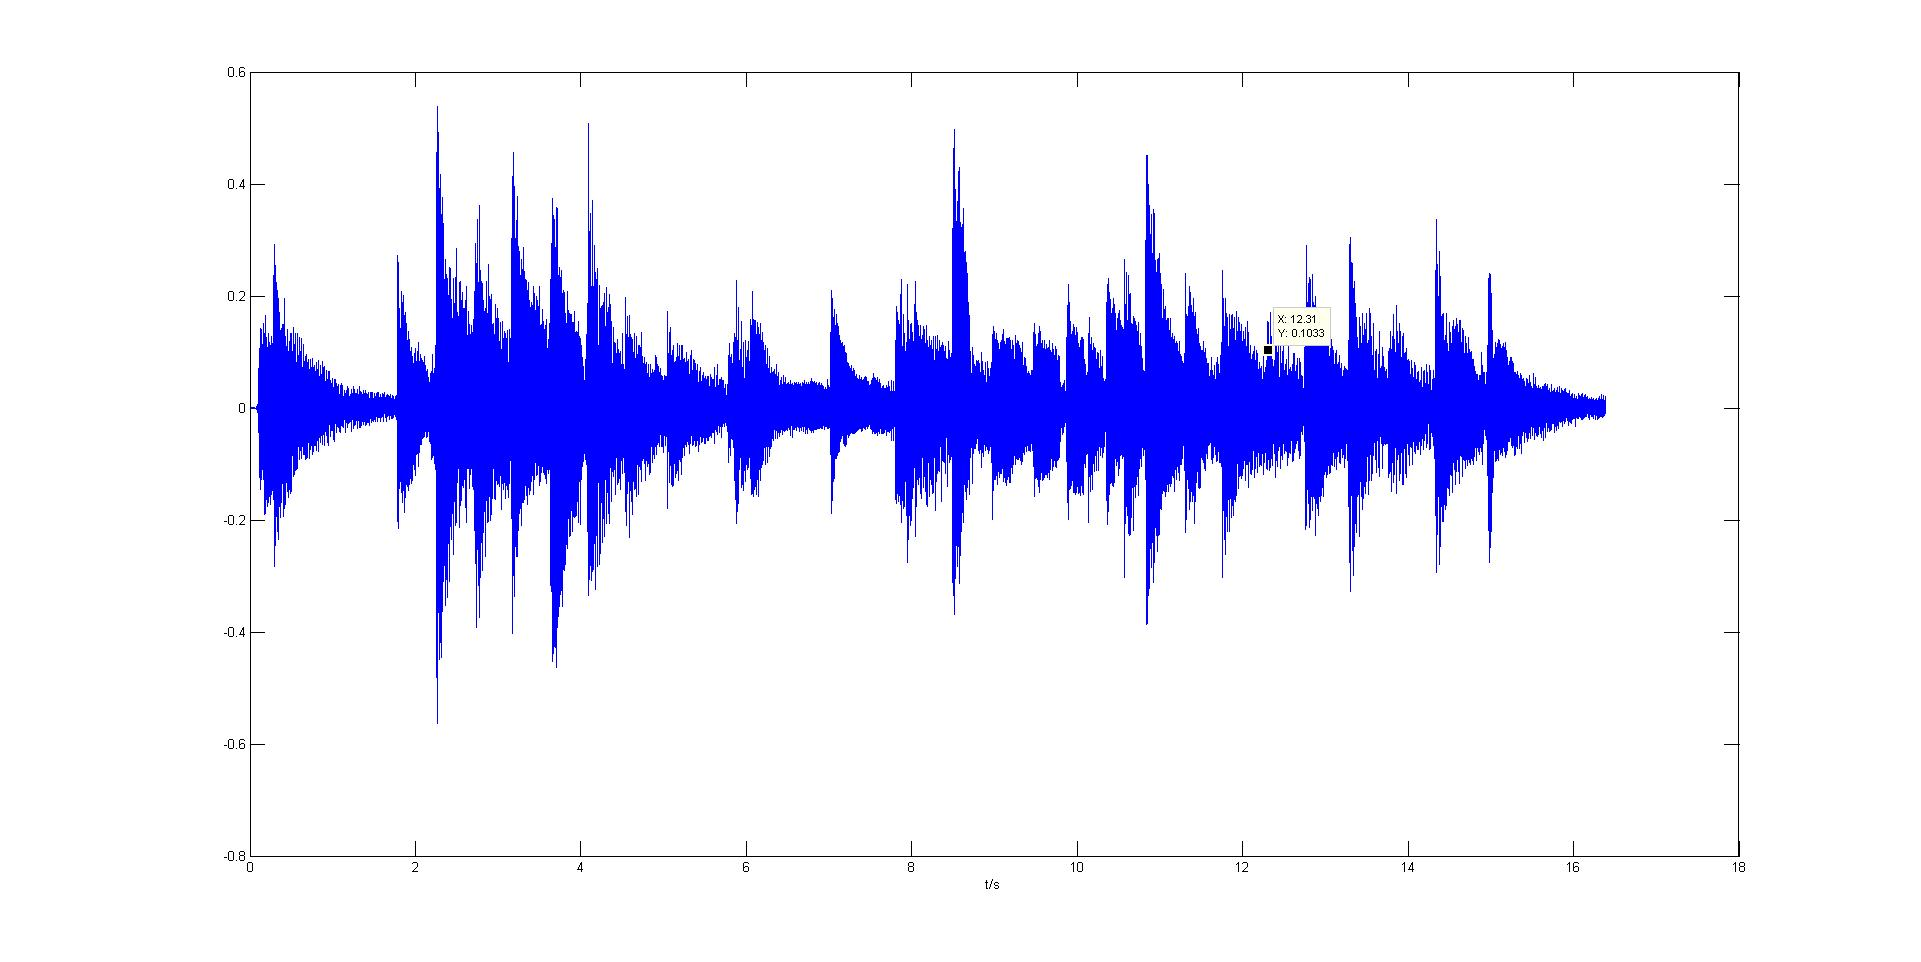
\includegraphics[width=0.8\textwidth]{fmt/1_9_2.jpg}\\
            \caption{fmt波形图\label{192}}
        \end{figure}


        因此,采用最基本的手工标定法,利用cooledit将音乐分为31段,分别存储在fmt (2).wav至fmt (32).wav 中,批处理获得各个音的音调即对应的的谐波强度。
				
			代码如下(anay.m,f\_f.m):
        \lstinputlisting[language=matlab]{fmt/anay.m}
        \lstinputlisting[language=matlab]{fmt/f_f.m}
        最终的得到的结果为图\ref{19sheet}(存储在变量freq和A中);
        \begin{figure}
            \centering
            \subfigure{
            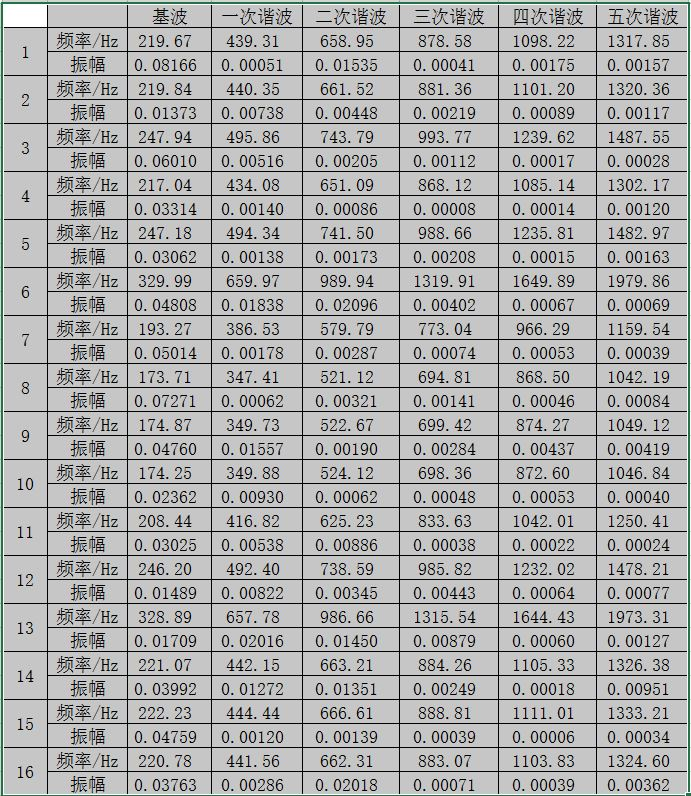
\includegraphics[width=0.6\textwidth]{fmt/1_9_sheet1.jpg}}
            \subfigure{
            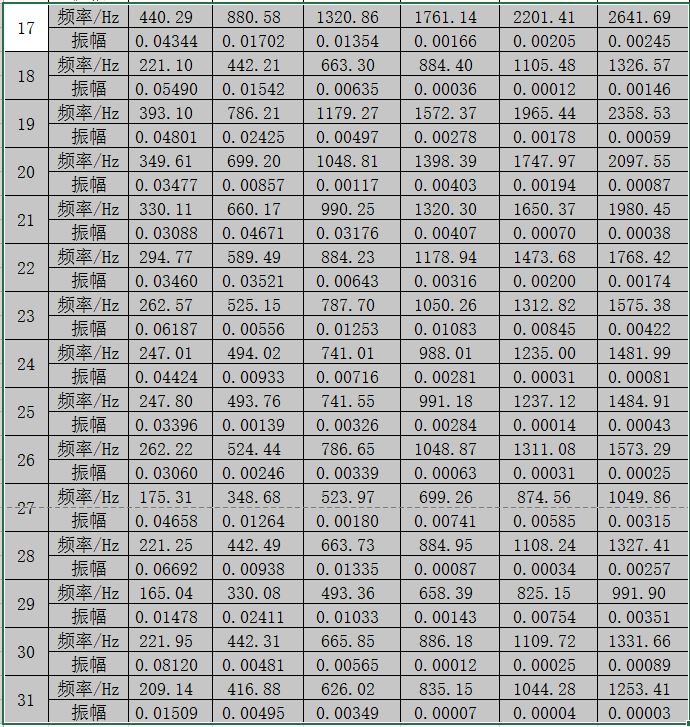
\includegraphics[width=0.6\textwidth]{fmt/1_9_sheet2.jpg}}
            \caption{fmt分析结果\label{19sheet}}
        \end{figure}

\section{
    基于傅里叶级数的合成音乐
}
\setcounter{subsection}{9} 
    \subsection{
            用 (7) 计算出来的傅里叶级数再次完成第 (4) 题,听一听是否像演奏 fmt.wav 的吉
            他演奏出来的?
        }
        思路:将谐波的振幅关系传给m\_note\_guitar函数,使产生的音有谐波分量。
        
        代码如下:(dfh\_guitar.m,m\_note\_guitar.m):

        \lstinputlisting[language=matlab]{fmt/dfh_guitar.m}
        \lstinputlisting[language=matlab]{fmt/m_note_guitar.m}

        思考:第一次做完后听起来并不像,但是这里的谐波分布和之前应该是一致的,为了更符合要求,我仿照图\ref{192}修改了包络,使得新的波形从图\ref{15}变为图\ref{110}.修改之后听起来确实像吉他了,但是还有一些奇怪的杂音。
        \begin{figure}
            \centering
            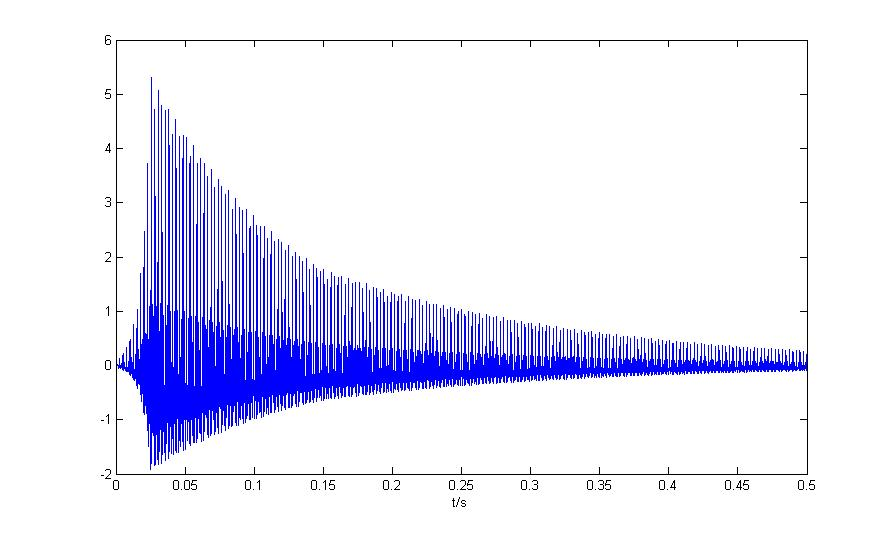
\includegraphics[width=0.8\textwidth]{fmt/1_10.jpg}\\
            \caption{新包络\label{110}}
        \end{figure}

    \subsection{
            也许(9) 还不是很像,因为对于一把泛音丰富的吉他而言,不可能每个音调对应的
            泛音数量和幅度都相同。但是通过完成第 (8) 题,你已经提取出 fmt.wav 中的很多音调,或
            者说,掌握了每个音调对应的傅里叶级数,大致了解了这把吉他的特征。现在就来演奏一
            曲《东方红》吧。提示:如果还是音调信息不够,那就利用相邻音调的信息近似好了,毕竟
            可以假设吉他的频响是连续变化的。
        }        

        代码如下:
        \lstinputlisting[language=matlab]{fmt/dfh_guitar_plus.m}

        生成的波形如图\ref{111}
        \begin{figure}
            \centering
            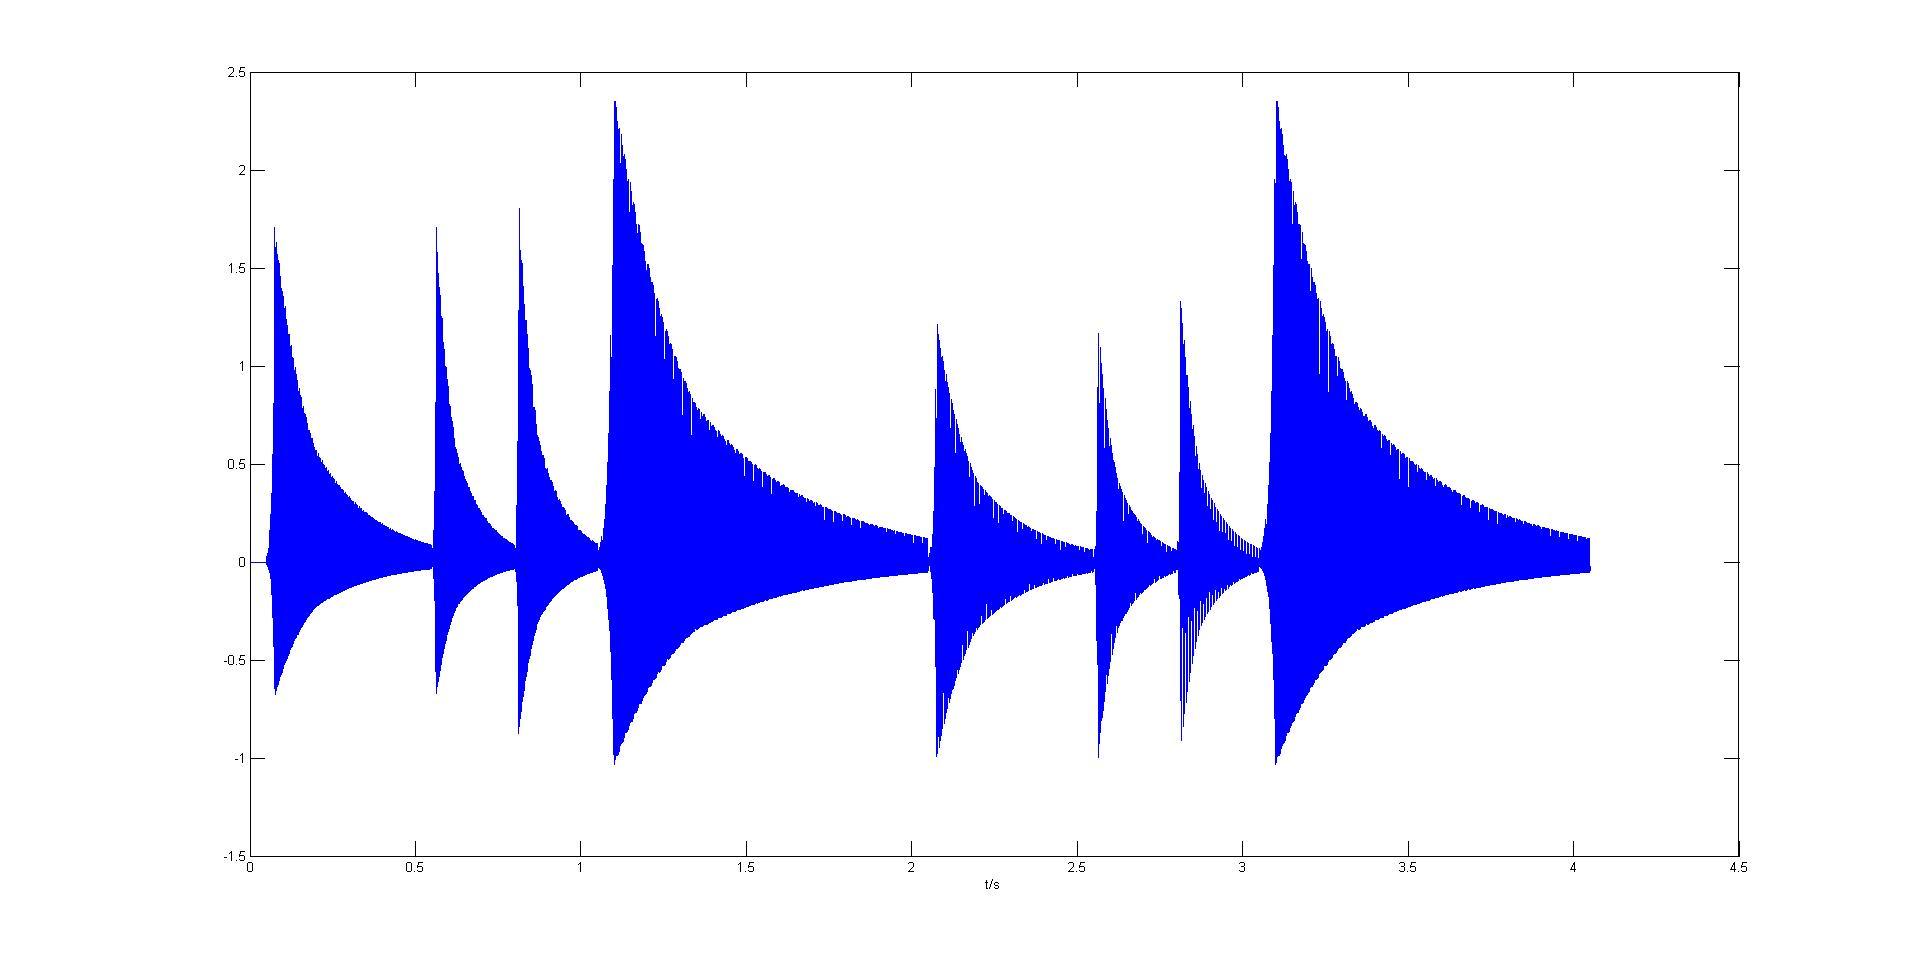
\includegraphics[width=0.8\textwidth]{fmt/1_11.jpg}\\
            \caption{生成的波形\label{111}}
        \end{figure}

        思考:听起来很像吉他了,但是两个长音中还是有杂音.
        但单独播放这个音的短音时并无杂音。所以这是拖得过长而导致的,
        给长音增加特殊的包络就能解决这一问题。
        和真实吉他不一样的是,这里缺乏和声和连音等修饰,所以听着有点单调。
        本题的难点在于将第(9)问的数据应用在这里,
        进行了较为复杂的运算才得以使用,使自己有了不小的提升。

    \subsection{
            现在只要你掌握了某乐器足够多的演奏资料,就可以合成出该乐器演奏的任何音
            乐,在学完本书后面内容之后,试着做一个图形界面把上述功能封装起来。
        }
       
        GUI界面如图\ref{112},其中内置了三首曲子:《东方红》《茉莉花》《致爱丽丝》;
        提供C大调和A大调两种音调;提供吉他、风琴(如第四题,但是仍使用吉他的包络)
        、电子音(只有基波)三种音色。

        在简谱栏中输入音符如1 2 3就是do re mi,11就是高八度的do,-6就是低八度的la,
        1.5就是$^b2$,-10表示是空音。可以演奏从-3到13的所有音(C大调,
        A大调为-5到15)在时间栏中输入各个音符对应的时间,
        样例乐谱选无,点击演奏就能听到音乐了。
     
        同时,用户可以点击分析音乐按钮,选择的一小段wav文件,
        程序会进行分析(无法进行分拍分析,只会当做一个音)。
        然后音色选择custom就能利用该段音乐的频谱特点模仿该音色。




        思考:本题的核心是GUI,主要的逻辑都需要做在按钮的callback函数中。
        因为给用户的反馈是按下按钮后出现的(发声)。
        这有几个难点,一个是空音,需要选择一个不会出现的数字。
        另一个是输入的处理,因为允许用户输入,所以必须增加限制以提高鲁棒性。

        有趣的是,当包络修改后,虽然和第(4)问采用了一样的谐波分布特性,
        但听着也有点像弦乐而非风琴,可见包络对于音色的影响也很明显。
        \begin{figure}
            \centering
            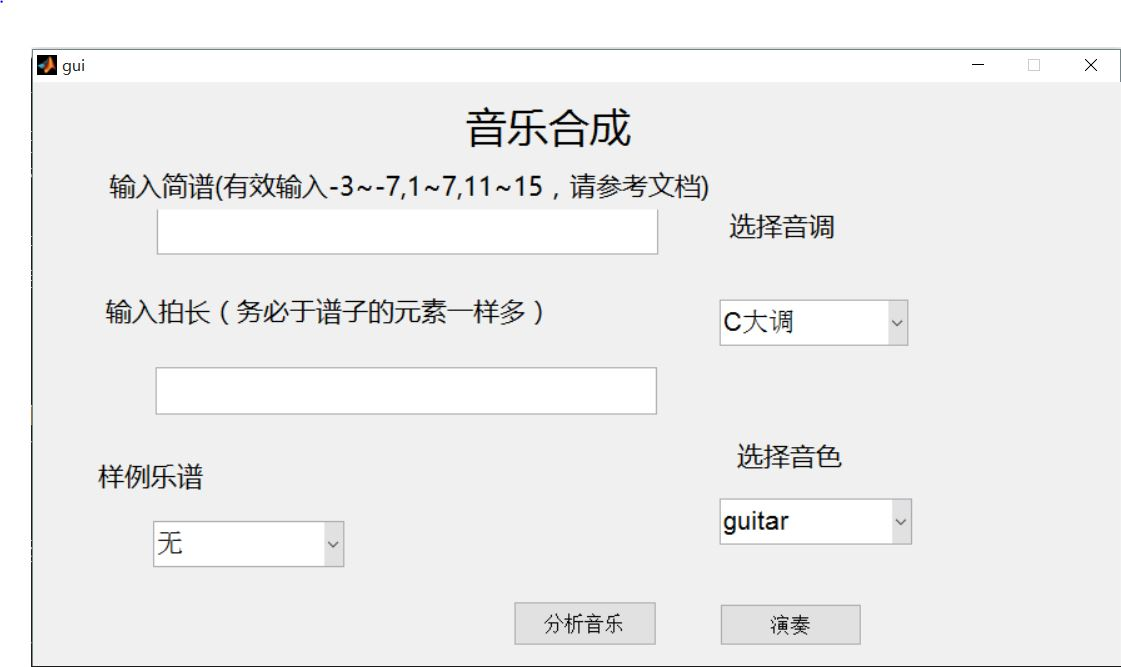
\includegraphics[width=0.8\textwidth]{fmt/1_12.jpg}\\
            \caption{GUI界面\label{112}}
        \end{figure}

        代码如下:(gui.m)
        \lstinputlisting[language=matlab]{fmt/gui.m}
\end{document}
